\begin{ex}%[2H2C2-5]
	Trong không gian $Oxyz$, cho $A(4;-2;6)$, $ B(2;4;2)$, $ M\in(\alpha)\colon x+2y-3z-7=0$ sao cho $\overrightarrow{MA}\cdot\overrightarrow{MB}$ nhỏ nhất. Tọa độ của $M$ bằng
	\choice
	{$M\left(\dfrac{29}{13};\dfrac{58}{13};\dfrac{5}{13}\right)$}
	{\True $ M(4;3;1)$}
	{$M(1;3;4)$}
	{$M\left(\dfrac{37}{3};-\dfrac{56}{3};\dfrac{68}{3}\right)$}
	\loigiai{
		\textbf{Cách 1}\\
\begin{center}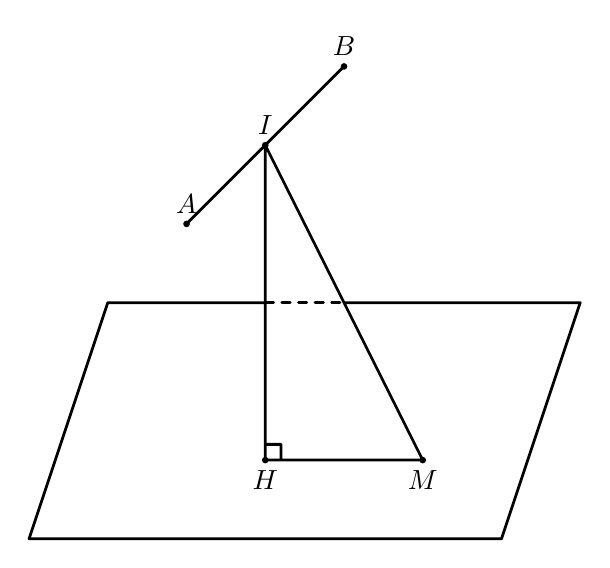
\begin{tikzpicture}[>=stealth,line join=round,line width=1pt, line cap=round]
\draw (0,1)--(-2,1)--(-3,-2)--(3,-2)--(4,1)--(1,1) (0,-1)--(2,-1)--(0,3)--(0,-1) (-1,2)--(1,4) (0,-0.8)--(0.2,-0.8)--(0.2,-1);
\draw[dashed] (0,1)--(1,1);
\fill (-1,2)node[above]{$A$}circle(1.2pt);
\fill (1,4)node[above]{$B$}circle(1.2pt);
\fill (0,3)node[above]{$I$}circle(1.2pt);
\fill (0,-1)node[below]{$H$}circle(1.2pt);
\fill (2,-1)node[below]{$M$}circle(1.2pt);
\end{tikzpicture}\end{center}
Gọi $I$ là điểm thỏa mãn $\overrightarrow{IA}+\overrightarrow{IB}=\overrightarrow{0}$. Suy ra $I$ là trung điểm của $AB$, do đó $I(3;1;4)$.\\  
Ta có $\overrightarrow{MA}\cdot\overrightarrow{MB}=(\overrightarrow{MI}+\overrightarrow{IA})\cdot(\overrightarrow{MI}+\overrightarrow{IB})=MI^2+\overrightarrow{MI}\cdot(\overrightarrow{IA}+\overrightarrow{IB})=MI^2$.\\
Gọi $H$ là hình chiếu của $I$ xuống mặt phẳng $(\alpha)$. Khi đó ta có 
$\overrightarrow{MA}\cdot\overrightarrow{MB}=MI^2\geq IH^2$.\\
Vậy giá trị nhỏ nhất của $\overrightarrow{MA}\cdot\overrightarrow{MB}$ là $IH^2$, đạt được khi $M\equiv H$.\\
Đường thẳng đi qua $I$ vuông góc với mặt phẳng $(\alpha)$ là $\Delta\colon \heva{&x=3+t\\&y=1+2t\\&z=4-3t.}$\\
Do $H$ là hình chiếu vuông góc của $I$ lên $(\alpha)$ nên $H=\Delta\cap (\alpha)$; suy ra $H(4;3;1)$.\\
\textbf{Cách 2}\\
	Gọi $ M(x;y;z)\in(\alpha)\Rightarrow x+2y-3z-7=0$.\\
	Ta có 	$\overrightarrow{MA}=(4-x;-2-y;6-z)$; $\overrightarrow{MB}=(2-x;4-y;2-z)$.
	\begin{align*} \overrightarrow{MA}\cdot\overrightarrow{MB}=&(4-x)(2-x)+(-2-y)(4-y)+(6-z)(2-z)\\ =&x^2+y^2+z^2-6x-2y-8z+12=(x-3)^2+(y-1)^2+(z-4)^2-12. \end{align*}
	Áp dụng bđt Bunhinacopxki - Cauchy - Schwarz.
	\begin{align*} &\left[1^2+2^2+\left(-3\right)^2\right]\left[\left(x-3\right)^2+\left(y-1\right)^2+\left(z-4\right)^2\right]\geq\left[x-3+2\left(y-1\right)-3\left(z-4\right)\right]^2\\ \Leftrightarrow &14\left[(x-3)^2+(y-1)^2+(z-4)^2\right]\geq{\left[x+2y-3z+7\right]^2}\\ \Leftrightarrow&(x-3)^2+(y-1)^2+(z-4)^2\geq\dfrac{\left(7+7\right)}{14}^2\\ \Leftrightarrow &(x-3)^2+(y-1)^2+(z-4)^2-12\geq 2.\end{align*}
		$ \min\left(\overrightarrow{MA}\cdot\overrightarrow{MB}\right)=2$ xảy ra khi và chỉ khi $$\heva{&x+2y-3z-7=0\\&\dfrac{x-3}{1}=\dfrac{y-1}{2}=\dfrac{z-4}{-3}}\Leftrightarrow\heva{&x=4\\&y=3\\&z=1}\Rightarrow M(4;3;1).$$
}
\end{ex}

\begin{ex}%[2H2C2-5]
	Trong không gian $Oxyz$, cho $A(1;-1;2)$, $B(-2,0,3)$, $C(0;1;-2)$. Gọi $M(a;b;c)$ là điểm thuộc mặt phẳng $(Oxy)$ sao cho biểu thức $S=\overrightarrow{MA}\cdot\overrightarrow{MB}+2\overrightarrow{MB}\cdot\overrightarrow{MC}+3\overrightarrow{MC}\cdot\overrightarrow{MA}$ đạt giá trị nhỏ nhất. Khi đó $ T=12a+12b+c$ có giá trị bằng
	\choice
	{$ T=3$}
	{$ T=-3$}
	{$ T=1$}
	{\True $ T=-1$}
	\loigiai
	{Xét 
		\begin{align*} S=&\overrightarrow{MA}\cdot\overrightarrow{MB}+2\overrightarrow{MB}\cdot\overrightarrow{MC}+3\overrightarrow{MC}\cdot\overrightarrow{MA}\\ =&(\overrightarrow{MI}+\overrightarrow{IA})(\overrightarrow{MI}+\overrightarrow{IB})+2(\overrightarrow{MI}+\overrightarrow{IB})(\overrightarrow{MI}+\overrightarrow{IC})+3(\overrightarrow{MI}+\overrightarrow{IC})(\overrightarrow{MI}+\overrightarrow{IA})\\
		=&6M{I^2}+\overrightarrow{MI}(4\overrightarrow{IA}+3\overrightarrow{IB}+5\overrightarrow{IC})+\overrightarrow{IA}\overrightarrow{IB}+2\overrightarrow{IB}\overrightarrow{IC}+3\overrightarrow{IC}\overrightarrow{IA}.\end{align*}
		Gọi I là điểm thỏa mãn $ 4\overrightarrow{IA}+3\overrightarrow{IB}+5\overrightarrow{IC}=\overrightarrow 0\Rightarrow I\left(\dfrac{-1}{6},\dfrac{1}{12},\dfrac{7}{12}\right)$.\\
		Mà: $\heva{&4\overrightarrow{IA}+3\overrightarrow{IB}+5\overrightarrow{IC}=\overrightarrow{0}\\ &\overrightarrow{IA}\cdot\overrightarrow{IB}+2\overrightarrow{IB}\cdot\overrightarrow{IC}+3\overrightarrow{IC}\cdot\overrightarrow{IA}=\text{const}.}$ \\
		Do đó $S_{\min}\Leftrightarrow MI_{\min}$, điều này xảy ra khi $M$ là hình chiếu của $I$ lên mặt $Oxy$.\\
		Ta dễ dàng tìm được tọa độ $M\left(-\dfrac{1}{6},\dfrac{1}{12},0\right)\Rightarrow T=12a+12b+c=-1$.}
\end{ex}

\begin{ex}%[2H2C2-5]
	Trong không gian với hệ trục tọa độ $Oxyz$, cho các điểm $A(4;1;5)$, $B(3;0;1)$, $C(-1;2;0)$ và điểm $ M(a;b;c)$ thỏa mãn $\overrightarrow{MA}\cdot\overrightarrow{MB}+2\overrightarrow{MB}\cdot\overrightarrow{MC}-5\overrightarrow{MC}\cdot\overrightarrow{MA}$ lớn nhất. Tính $P=a-2b+4c$.
	\choice
	{$P=23$}
	{$P=31$}
	{$P=11$}
	{\True $P=13$}
	\loigiai
{Đặt  $Q=\overrightarrow{MA}\cdot\overrightarrow{MB}+2\overrightarrow{MB}\cdot\overrightarrow{MC}-5\overrightarrow{MC}\cdot\overrightarrow{MA}$.
	\begin{align*}	&\left(\overrightarrow{MA}-\overrightarrow{MB}\right)^2=MA^2+MB^2-2\overrightarrow{MA}\cdot\overrightarrow{MB}\Rightarrow\overrightarrow{MA}\cdot\overrightarrow{MB}=\dfrac{1}{2}\left(MA^2+MB^2-AB^2\right)\\		&\left(\overrightarrow{MB}-\overrightarrow{MC}\right)^2=MB^2+MC^2-2\overrightarrow{MB}\cdot\overrightarrow{MC}\Rightarrow 2\overrightarrow{MB}\cdot\overrightarrow{MC}=MB^2+MC^2-BC^2\\
	&\left(\overrightarrow{MC}-\overrightarrow{MA}\right)^2=MC^2+MA^2-2\overrightarrow{MC}\cdot\overrightarrow{MA}\Rightarrow\overrightarrow{MC}\cdot\overrightarrow{MA}=\dfrac{1}{2}\left(MC^2+MA^2-AC^2\right).\end{align*}
Từ đây, ta suy ra 
\begin{align*} Q=&\overrightarrow{MA}\cdot\overrightarrow{MB}+2\overrightarrow{MB}\cdot\overrightarrow{MC}-5\overrightarrow{MC}\cdot\overrightarrow{MA}\\
 =&\dfrac{1}{2}\left(MA^2+MB^2-AB^2\right)+MB^2+MC^2-BC^2-\dfrac{5}{2}\left(MC^2+MA^2-AC^2\right)\\ =&-2MA^2+\dfrac{3}{2}MB^2-\dfrac{3}{2}MC^2-\dfrac{1}{2}AB^2-BC^2+\dfrac{5}{2}AC^2.\end{align*}
Gọi $ E$ là điểm thỏa mãn $-2\overrightarrow{EA}+\dfrac{3}{2}\overrightarrow{EB}-\dfrac{3}{2}\overrightarrow{EC}=\overrightarrow{0}\Leftrightarrow\overrightarrow{EA}=\dfrac{3}{4}\overrightarrow{CB}\Leftrightarrow E\left(1;\dfrac{5}{2};\dfrac{17}{4}\right)$.\\

Ta có 
\begin{align*} Q=&-2MA^2+\dfrac{3}{2}MB^2-\dfrac{3}{2}MC^2-\dfrac{1}{2}AB^2-BC^2+\dfrac{5}{2}AC^2\\
	=&-2\left(\overrightarrow{ME}+\overrightarrow{EA}\right)^2+\dfrac{3}{2}\left(\overrightarrow{ME}+\overrightarrow{EB}\right)^2-\dfrac{3}{2}\left(\overrightarrow{ME}+\overrightarrow{EC}\right)^2-\dfrac{1}{2}AB^2-BC^2+\dfrac{5}{2}AC^2\\
	=&-2ME^2-2EA^2+\dfrac{3}{2}EB^2-\dfrac{3}{2}EC^2-\dfrac{1}{2}AB^2-BC^2+\dfrac{5}{2}AC^2\\
	\leq&-2EA^2+\dfrac{3}{2}EB^2-\dfrac{3}{2}EC^2-\dfrac{1}{2}AB^2-BC^2+\dfrac{5}{2}AC^2.
\end{align*}
Vì $T=-2EA^2+\dfrac{3}{2}EB^2-\dfrac{3}{2}EC^2\le-2EA^2+\dfrac{3}{2}EB^2-\dfrac{3}{2}EC^2-\dfrac{1}{2}AB^2-BC^2+\dfrac{5}{2}AC^2=\text{const}$ không đổi nên $Q$ đạt giá trị lớn nhất khi $ME=0\Rightarrow M\equiv E$.\\
Vậy $M\left(1;\dfrac{5}{2};\dfrac{17}{4}\right)\Rightarrow P=a-2b+4c=13$.}
\end{ex}

\begin{ex} %[2H2C2-5]
	Trong không gian $Oxyz$, cho ba điểm $A(-8;1;1)$, $B(2;1;3)$ và $C(6;4;0)$. Một điểm $M$ di động trong không gian sao cho $\overrightarrow{MA}\cdot\overrightarrow{MC}=\overrightarrow{MA}\cdot\overrightarrow{MB}+34$. Biết rằng $\left|MA-MB\right|$ đạt giá trị lớn nhất khi điểm $M$ trùng với điểm $M_0(x_0;y_0;z_0)$. Tích số $x_0y_0z_0$ bằng.
	\choice
	{$16$}
	{\True $18$}
	{$14$}
	{$12$}
\loigiai{Gọi $M=(a;b;c)$.\\
	Ta có $\overrightarrow{MA}\cdot\overrightarrow{MC}=\overrightarrow{MA}\cdot\overrightarrow{MB}+34\Leftrightarrow\overrightarrow{MA}\left(\overrightarrow{MC}-\overrightarrow{MB}\right)=34\Leftrightarrow\overrightarrow{MA}\cdot\overrightarrow{BC}=34$.\\
	Mặt khác $\overrightarrow{MA}=(-8-a;1-b;1-c)$, $\overrightarrow{BC}=(4;3;-3)$.\\
	Suy ra $4(-8-a)+3(1-b)-3(1-c)=34\Leftrightarrow-4a-3b+3c-66=0$.\\
	Vậy $M\in (P)$ có phương trình $-4x-3y+3z-66=0$.\\
	Ký hiệu $f(M)=f(x;y;z)=-4x-3y+3z-66$, với $M(x;y;z)$.\\
	Ta có $f(A)\cdot f(B)=(-4(-8)-3.1+3.1-66)(-4.2-3.1+3.3-66)=2312>0$.\\
	Suy ra điểm $A(-8;1;1)$ và điểm $B(2;1;3)$ nằm về cùng 1 phía so với mặt phẳng $(P)$.\\
	Khi đó $\left|MA-MB\right|\leq AB$ (tính chất 3 cạnh của tam giác) suy ra $\left|MA-MB\right|$ đạt giá trị lớn nhất khi $M$, $A$, $B$ thẳng hàng và $M$ nằm ngoài đoạn thẳng $AB$ hay $M$ là giao điểm của đường thẳng $AB$ với mặt phẳng $(P)$.\\
	Đường thẳng $AB$ có véc tơ chỉ phương $\overrightarrow{AB}=(10,0,2)$ và qua điểm $B(2,1,3)$ nên có phương trình $\heva{&x=2+5t\\&y=1\\&z=3+t.}$\\
	Suy ra $-4(2+5t)-3+3(3+t)-66=0\Leftrightarrow t=-4$.\\
	Vậy $M(-18,1,-1)$ hay $x_0y_0z_0=18$.
	}
\end{ex}
\Closesolutionfile{ans}
\indapan{6}{ans/ans-C5B3CD5-LC}

\TNSA
\Opensolutionfile{ans}[ans/ans-C5B3CD5-KQ]
\begin{ex} %[2H2C2-5]
	Trong không gian với hệ tọa độ $Oxyz$ cho $A(3;2;1)$, $B(-2;3;6)$. Điểm $ M(x_M;y_M;z_M)$ thay đổi thuộc mặt phẳng $(Oxy)$. Tìm giá trị của biểu thức $ T=x_M+y_M+z_M$ khi $\left|\overrightarrow{MA}+3\overrightarrow{MB}\right|$ nhỏ nhất.
\shortans[]{$2$}
\loigiai{
	Gọi điểm $H$ thỏa mãn $\overrightarrow{HA}+3\overrightarrow{HB}=\overrightarrow{0}$ khi đó $\heva{&{x_H}=\dfrac{x_A+3x_B}{1+3}\\
	&{y_H}=\dfrac{y_A+3y_B}{1+3}\\
	&{z_H}=\dfrac{z_A+3z_B}{1+3}}\Rightarrow H\left(-\dfrac{3}{4};\dfrac{11}{4};\dfrac{19}{4}\right)$.\\
	Ta có $\left|\overrightarrow{MA}+3\overrightarrow{MB}\right|=4|\overrightarrow{MH}|=4MH$.\\
	Biểu thức $\left|\overrightarrow{MA}+3\overrightarrow{MB}\right|$ đạt giá trị nhỏ nhất khi và chỉ khi $MH$ nhỏ nhất, khi đó $M$ là hình chiếu của $H$ lên mặt phẳng $Oxy$.\\	
Ta có $H\left(-\dfrac{3}{4};\dfrac{11}{4};\dfrac{19}{4}\right)\Rightarrow M\left(-\dfrac{3}{4};\dfrac{11}{4};0\right)$.\\
	Vậy $T=x_M+y_M+z_M$$=-\dfrac{3}{4}+\dfrac{11}{4}+0=2$.}
\end{ex}
	
\begin{ex}%[2H2C2-5]
Trong không gian với hệ trục $Oxyz$, cho các điểm $A(-1;2;3)$, $B(6,-5,8)$ và $\overrightarrow{OM}=a\overrightarrow{i}+b\overrightarrow{k}$, trong đó $a$, $b$ là các số thực luôn thay đổi. Nếu $\left|\overrightarrow{MA}-2\overrightarrow{MB}\right|$ đạt giá trị nhỏ nhất thì giá trị $a-b$ bằng bao nhiêu ?
\shortans[]{$0$}
\loigiai{
Ta có $\overrightarrow{OM}=a\overrightarrow{i}+b\overrightarrow{k}\Rightarrow M(a;0;b)$.\\
Ta tính được 
$\heva{&\overrightarrow{MA}=(-1-a;2;3-b)\\&\overrightarrow{MB}=(6-a;-5;8-b)}\Rightarrow \overrightarrow{MA}-2\overrightarrow{MB}=(a-13;12;b-13)$. \\
Suy ra, $\left|\overrightarrow{MA}-2\overrightarrow{MB}\right|^2=(a-13)^2+144+(b-13)^2\geq 144$, do đó $\min \left|\overrightarrow{MA}-2\overrightarrow{MB}\right|=12$ đạt được khi $\heva{&a=13\\&b=13}$. Vậy $a-b=0$.
}
\end{ex}

\begin{ex}%[2H2C2-5]
Trong không gian với hệ tọa độ $Oxyz$, cho ba điểm $ A(-1;2;5)$, $B(3;-1;0)$, $C(-4;0;-2)$. Gọi $I$ là điểm trên mặt phẳng $(Oxy)$ sao cho biểu thức $\left|\overrightarrow{IA}-2\overrightarrow{IB}+3\overrightarrow{IC}\right|$ đạt giá trị nhỏ nhất. Tính khoảng cách từ $I$ đến mặt phẳng $(P)\colon 4x+3y+2=0$.
\shortans[]{$6$}
\loigiai{
Gọi $M$ là điểm thỏa $\overrightarrow{MA}-2\overrightarrow{MB}+3\overrightarrow{MC}=\overrightarrow{0}\Rightarrow M\left(-\dfrac{19}{2};2;-\dfrac{1}{2}\right)$.\\
Ta có: \begin{align*}\left|\overrightarrow{IA}-2\overrightarrow{IB}+3\overrightarrow{IC}\right|=&\left|\overrightarrow{IM}+\overrightarrow{MA}-2\overrightarrow{IM}-2\overrightarrow{MB}+3\overrightarrow{IM}+3\overrightarrow{MC}\right|\\ =&\left|2\overrightarrow{IM}+\left(\overrightarrow{MA}-2\overrightarrow{MB}+3\overrightarrow{MC}\right)\right|=2\left|\overrightarrow{IM}\right|=2IM.
\end{align*}
Biểu thức $\left|\overrightarrow{IA}-2\overrightarrow{IB}+3\overrightarrow{IC}\right|$ đạt giá trị nhỏ nhất $\Leftrightarrow IM$ nhỏ nhất, điều này tương đương $ I$ là hình chiếu vuông góc của $ M$ lên $\left(Oxy\right)$. Do đó $I\left(-\dfrac{19}{2};2;0\right)$.\\
Khoảng cách từ điểm $ I$ đến mặt phẳng $(P)$ là $\mathrm{d}(I;(P))=\dfrac{\left|4\cdot\left(-\dfrac{19}{2}\right)+3\cdot 2+2\right|}{\sqrt{4^2+3^2}}=6$.
}
\end{ex}
\begin{ex}%[2H2C2-5]
	Trong không gian $Oxyz$, cho hai điểm $A(1;2;1)$; $B(2;-1;3)$ và điểm $M(a;b;0)$ sao cho $MA^2+MB^2$ nhỏ nhất. Tính giá trị của $a+b$ bằng 
\shortans[]{$2$}
\loigiai{
Gọi $I$ là trung điểm của $AB$, khi đó $\overrightarrow{IA}+\overrightarrow{IB}=\overrightarrow{0}$ và $I\left(\dfrac{3}{2};\dfrac{1}{2};2\right)$.\\
Ta có $MA^2+MB^2=2IM^2+IA^2+IB^2=2IM^2+\dfrac{AB^2}{2}=IM^2+7$.\\
Để $MA^2+MB^2$ nhỏ nhất thì $MI$ nhỏ nhất, mà $M(a;b;0)\in (Oxy)$. Do đó $M$ là hình chiếu vuông góc của $I$ lên $(Oxy)$. Suy ra $M\left(\dfrac{3}{2};\dfrac{1}{2};0\right)$.\\
 Như vậy $a=\dfrac{3}{2},b=\dfrac{1}{2}\Rightarrow a+b=\dfrac{3}{2}+\dfrac{1}{2}=2$ .}
	\end{ex}
\begin{ex}%[2H2C2-5]
Trong không gian cho ba điểm $A(1;1;1)$, $B(-1;2;1)$, $C(3;6;-5)$. Điểm $M(a,b,c)$ thuộc mặt phẳng $(Oxy)$ sao cho $MA^2+MB^2+MC^2$ đạt giá trị nhỏ nhất. Giá trị của $ab$ bằng
\shortans[]{$3$}
\loigiai{
Lấy $ G(1;3;-1)$ là trọng tâm của tam giác $ABC$.\\
Ta có $MA^2+MB^2+MC^2=3MG^2+GA^2+GB^2+GC^2$.\\
Do đó $MA^2+MB^2+MC^2$ bé nhất khi $MG$ bé nhất hay $M$ là hình chiếu của điểm $G$ lên mặt phẳng $Oxy$. Vậy $ M(1;3;0)$.}
\end{ex}
\begin{ex}%[2H2C2-5]
Trong không gian $Oxyz$, cho $A(0;1;2)$, $B(1;1;0)$, $C(3;0;1)$ và mặt phẳng $(Q)\colon x+y+z-5=0$. Xét điểm $M$ thay đổi thuộc $(Q)$. Giá trị nhỏ nhất của biểu thức $MA^2+MB^2+MC^2$ bằng $\dfrac{a}{b}$ với $a$, $b$ là hai số tự nhiên nguyên tố cùng nhau. Giá trị $a+b$ bằng
\shortans[]{$37$}
\loigiai{
	Gọi điểm $G$ thỏa $\overrightarrow{GA}+\overrightarrow{GB}+\overrightarrow{GC}=\overrightarrow 0$, suy ra $G\left(\dfrac{4}{3};\dfrac{2}{3};1\right)$.\\
	Khi đó $P=MA^2+MB^2+MC^2=3MG^2+GA^2+GB^2+GC^2$\\
	$\Rightarrow P\geq 3\left[\mathrm{d}(G,(Q))\right]^2+GA^2+GB^2+GC^2$.\\
	Dấu bằng xảy ra khi $M$ là hình chiếu của $G$ lên mặt phẳng $(Q)$.\\
	Ta có 
$\heva{&d\left(G,(Q)\right)=\dfrac{\left|\dfrac{4}{3}+\dfrac{2}{3}+1-5\right|}{\sqrt 3}=\dfrac{2}{\sqrt 3}\\
&\overrightarrow{GA}=\left(-\dfrac{4}{3};\dfrac{1}{3};1\right)\Rightarrow G{A^2}=\dfrac{26}{9},\\ &\overrightarrow{GB}=\left(-\dfrac{1}{3};\dfrac{1}{3};-1\right)\Rightarrow G{B^2}=\dfrac{11}{9},\\ &\overrightarrow{GC}=\left(\dfrac{5}{3};-\dfrac{2}{3};0\right)\Rightarrow G{C^2}=\dfrac{29}{9}.}$\\
Vậy $\min P=\dfrac{34}{3}$ khi $M$ là hình chiếu của $G$ lên mặt phẳng $(Q)$.}
\end{ex}
\begin{ex} %[2H2C2-5]
Trong không gian với hệ tọa độ $Oxyz$, cho bốn điểm $A(2;4;-1)$, $B(1;4;-1)$, $C(2;4;3)$ và $D(2;2;-1)$, biểu thức $MA^2+MB^2+MC^2+MD^2$ đạt giá trị nhỏ nhất khi $M(x;y;z)$. Giá trị $x+y+z$ bằng
\shortans[]{$5{,}25$}
\loigiai{
Chọn điểm $I$ sao cho $\overrightarrow{IA}+\overrightarrow{IB}+\overrightarrow{IC}+\overrightarrow{ID}=\overrightarrow{0}$. Khi đó $I\left(\dfrac{7}{4};\dfrac{7}{2};0\right)$.\\
Ta có $MA^2+MB^2+MC^2+MD^2=4MI^2+IA^2+IB^2+IC^2+ID^2$.\\
Do $I$, $A$, $B$, $C$, $D$ cố định nên $IA^2+IB^2+IC^2+ID^2$ không đổi.\\
Do đó để $MA^2+MB^2+MC^2+MD^2$ đạt giá trị nhỏ nhất thì $MI$ nhỏ nhất, tức là $MI=0$, hay $M\equiv I$.\\
Vậy $I\left(\dfrac{7}{4};\dfrac{7}{2};0\right)$ nên $x+y+z=\dfrac{21}{4}$.
}
\end{ex}
\begin{ex} %[2H2C2-5]
Trong không gian $Oxyz$, cho ba điểm $A(0;0;1)$, $B(-1;1;0)$, $C(1;0;-1)$. Điểm $M$ di động trên mặt phẳng $(P)\colon 2x+2y-z+2=0$. Biết giá trị nhỏ nhất của $3MA^2+2MB^2+MC^2$ là $\dfrac{a}{b}$ với $a$, $b$ là hai số tự nhiên nguyên tố cùng nhau. Giá trị $a-b$ bằng
\shortans[]{$55$}
\loigiai{
Gọi $I$ là điểm thỏa mãn $3\overrightarrow{IA}+2\overrightarrow{IB}+\overrightarrow{IC}=\overrightarrow{0}\Rightarrow I\left(-\dfrac{1}{6};\dfrac{1}{3};\dfrac{1}{3}\right)$.\\
Ta có $3MA^2+2MB^2+MC^2=3IA^2+2IB^2+IC^2+6IM^2$.\\
Do đó $3MA^2+2MB^2+MC^2$ nhỏ nhất khi và chỉ khi $IM$ nhỏ nhất, tương đương $M$ là hình chiếu của $I$ trên $(P)$.\\
Khi đó $\min IM=\mathrm{d}(I,(P))=\dfrac{2}{3}$, suy ra $\min (3MA^2+2MB^2+MC^2)=\dfrac{61}{6}$.
%Phương trình đường thẳng đi qua $I$ vuông góc với mặt phẳng $(P)$ là $\Delta\colon \heva{&x=-\dfrac{1}{6}+2t\\&y=\dfrac{1}{3}+2t\\&z=\dfrac{1}{3}-t}$.\\
%$M$ là hình chiếu của $I$ lên $(P)$ nên $M=\Delta\cap (P)$, suy ra $M\left(-\dfrac{11}{18};-\dfrac{1}{9};\dfrac{5}{9}\right)$
% $\Rightarrow M\left(-\dfrac{11}{18};-\dfrac{1}{9};\dfrac{5}{9}\right)$ 
}
\end{ex}

\begin{ex} %[2H2C2-5]
Trong không gian $Oxyz$, cho ba điểm $A(2;-2;4)$, $B(-3;3;-1)$, $C(-1;-1;-1)$ và mặt phẳng $(P)\colon 2x-y+2z+8=0$. Xét điểm $M$ thay đổi thuộc $(P)$, tìm giá trị nhỏ nhất của biểu thức $T=2MA^2+MB^2-MC^2$.
\shortans[]{$102$}
\loigiai{
Gọi $I$ là điểm thỏa $2\overrightarrow{IA}+\overrightarrow{IB}-\overrightarrow{IC}=\overrightarrow{0}\Rightarrow I(1;0;4)$.\\
Ta có $T=2MA^2+MB^2-MC^2=2MI^2+(2IA^2+IB^2-IC^2)$.\\
Để $T$ nhỏ nhất thì $ 2MI^2$ nhỏ nhất $\Leftrightarrow MI$ ngắn nhất $M$ là hình chiếu của điểm $I$ lên $(P)$. Khi đó $MI=\mathrm{d}\left(I,(P)\right)=6$ và $2IA^2+IB^2-IC^2=30$, suy ra $\min T=102$.}
\end{ex}

\begin{ex} %[2H2C2-5]
Trong không gian với hệ trục tọa độ $Oxyz$, cho ba điểm $A(1;4;5)$, $B(3;4;0)$, $C(2;-1;0)$ và mặt phẳng $(\alpha)\colon 3x-3y-2z-12=0$ Gọi $M(a;b;c)$ thuộc $(\alpha)$ sao cho $MA^2+MB^2+3MC^2$ đạt giá trị nhỏ nhất. Tính tổng $S=a+b+c$.
\shortans[]{$3$}
\loigiai{
Gọi $I$ là điểm thỏa $\overrightarrow{IA}+\overrightarrow{IB}+3\overrightarrow{IC}=\overrightarrow{0}\Rightarrow I(2;1;1).$\\
Mặt khác $MA^2+MB^2+3MC^2=5MI^2+IA^2+IB^2+3IC^2$.\\
Vì $I$, $A$, $B$, $C$ cố định nên $ IA^2+IB^2+3IC^2$ không đổi.\\
Do đó $ MA^2+MB^2+3MC^2$ nhỏ nhất $\Leftrightarrow MI^2$ nhỏ nhất $\Leftrightarrow MI$ nhỏ nhất. Điều này xảy ra khi $M$ là hình chiếu của $I$ trên mặt phẳng $(\alpha)$.\\
Phương trình đường thẳng $\Delta$ qua $I$ và vuông góc với mặt phẳng $(\alpha)$ là $\heva{&x=2+3t\\&y=1-3t\\&z=1-2t.}$\\
$M$ là hình chiếu của $I$ lên $(\alpha)$ nên $M=\Delta\cap (\alpha)$; suy ra $M\left(\dfrac{7}{2};-\dfrac{1}{2};0\right)$.\\
Vậy $S=a+b+c=3$.}
\end{ex}

\begin{ex} %[2H2C2-5]
Trong không gian tọa độ $Oxyz$, cho hai điểm $A(3;-2;2)$, $B(-2;2;0)$ và mặt phẳng $(P)\colon 2x-y+2z-3=0$. Xét các điểm $M$, $N$ di động trên $(P)$ sao cho $MN=1$. Tính giá trị nhỏ nhất của biểu thức $2AM^2+3BN^2$. (kết quả làm tròn đế 1 chữ số thập phân).
\shortans[]{$49{,}8$}
\loigiai{
Gọi $H$, $K$ lần lượt là hình chiếu của $A$, $B$ trên mặt phẳng $(P)$, khi đó ta tìm được $AH=BK=3$, $H(1;-1;0)$, $K(0;1;2)$ nên $HK=3$.\\
Đặt $HM=t$ ta có $HM+MN+NK\geq HK=3\Rightarrow NK\geq 2-t$\\
\begin{align*} 2AM^2+3BN^2= &2(AH^2+HM^2)+3(BK^2+KN^2)\\ \geq &45+2t^2+(2-t)^2=\left(\sqrt 3 t-\dfrac{2}{\sqrt 3}\right)^2+\dfrac{143}{3}\ge\dfrac{143}{3}.\end{align*}
Dấu bằng xảy ra khi $ M$, $N$ thuộc đoạn thẳng $HK$.\\
Vậy giá trị nhỏ nhất của biểu thức $ 2AM^2+3BN^2$ bằng $\dfrac{143}{3}\approx49{,}8$.}
\end{ex}

\begin{ex} %[2H2C2-5]
Trong không gian với hệ tọa độ $Oxyz$, cho điểm $A(a;b;c)$ với $a$, $b$, $c$ là các số thực dương thỏa mãn $5(a^2+b^2+c^2)=9(ab+2bc+ca)$ và $Q=\dfrac{a}{b^2+c^2}-\dfrac{1}{(a+b+c)^3}$ có giá trị lớn nhất. Gọi $M$, $N$, $P$ lần lượt là hình chiếu vuông góc của $A$ lên các tia $Ox$, $Oy$, $Oz$. Khi đó phương trình mặt phẳng $(MNP)$ là $mx+ny+pz-1=0$. Giá trị $m+np$ bằng
\shortans[]{$147$}
\loigiai{
Đặt $t=b+c$, khi đó $t>0$; $b^2+c^2\geq\dfrac{t^2}{2}$; $bc\leq\dfrac{t^2}{4}$.\\
\begin{align*} &5(a^2+b^2+c^2)=9(ab+2bc+ca)\\ \Leftrightarrow &5a^2+5\left(b+c\right)^2-9a\left(b+c\right)=28bc\\ \Rightarrow &5a^2+5t^2-9at\leq 7t^2\Leftrightarrow(5a+t)(a-2t)\leq 0\Leftrightarrow a\leq 2t.\end{align*}
Vậy $Q\leq\dfrac{4}{t}-\dfrac{1}{27t^3}=f(t)$ với $t > 0$.\\
Ta có  $f'(t)=-\dfrac{4}{t^2}+\dfrac{1}{9t^4}$, $\,\,$ $f'(t)=0\Leftrightarrow t=\dfrac{1}{6}$ (vì $t>0$).\\
Ta có bảng biến thiên
\begin{center}\begin{tikzpicture}[>=stealth]
	\tkzTabInit[nocadre=false,lgt=1.3,espcl=2,deltacl=0.5]{$x$/1.2 ,$f'(t)$/.9,$f(t)$/2}
	{$0$ , $\dfrac{1}{6}$ , $+\infty$}
	\tkzTabLine{ , + , $0$ , - , }
	\tkzTabVar{-/$-\infty$ , +/$16$ , -/$0$}
\end{tikzpicture}\end{center}
Vậy $\max Q=16$ đạt được khi $a=\dfrac{1}{3}$; $b=c=\dfrac{1}{12}$.\\
Suy ra tọa độ điểm $A\left(\dfrac{1}{3};\dfrac{1}{12};\dfrac{1}{12}\right)$; tọa độ các điểm $M\left(\dfrac{1}{3};0;0\right)$; $N\left(0;\dfrac{1}{12};0\right)$; $P\left(0;0;\dfrac{1}{12}\right)$.\\
Phương trình mặt phẳng $\left(MNP\right)$ $\dfrac{x}{\dfrac{1}{3}}+\dfrac{y}{\dfrac{1}{12}}+\dfrac{z}{\dfrac{1}{12}}=1$ $\Leftrightarrow 3x+12y+12z-1=0$.\\ Suy ra $m+np=147$.}
\end{ex}
\Closesolutionfile{ans}
\indapan{6}{ans/ans-C5B3CD5-KQ}
